\section{模型建立与求解}

\subsection{问题一}

\subsubsection{模型的构建和分析}

在开始之前,我们需要先构建整个装置的物理模型。
以海平面为参考系。

当装置在水中静止时,对质量为 $m$ 的振子进行受力分析,则其受到的重力和受到弹簧弹力合力为零。
记以铅直向上为正方向,重力加速度为 $g$,记此时振子位移为 0,记此时弹簧压缩量为 $x_0$,弹簧的刚度为 $k$,则有 
\begin{equation}
    kx_0-mg=0 
    \label{oscilator}
\end{equation}

考虑在 $t$ 时刻,浮子位移 $x_1$,振子位移 $x_2$,正方向同前定义。
记阻尼器的阻尼系数为 $c$,对振子受力分析,如图 \ref{force-analysis} 左所示。我们有
\begin{equation}
    m\dfrac{\dif^2x_2}{\dif t^2}=k(x_1-x_2+x_0)+c(\dfrac{\dif{x_1}}{\dif{t}}-\dfrac{\dif{x_2}}{\dif{t}})-mg
\end{equation}
其中,$\dfrac{\dif^2 x_i}{\dif t^2}$ 即为瞬时加速度,$\dfrac{\dif x_i}{\dif t}$ 即为瞬时速度。

与此同时,我们对浮子进行受力分析,如图 \ref{force-analysis} 右所示。
记海水的兴波阻尼系数为 $c_0$,附加质量为 $m_0$,浮子质量为 $M$,波浪激励力为 $F$,有 
\begin{equation}
    M\dfrac{\dif^2x_1}{\dif t^2}=F+F_\text{浮}-Mg-k(x_1-x_2+x_0)-c(\dfrac{\dif{x_1}}{\dif{t}}-\dfrac{\dif{x_2}}{\dif{t}})-c_0\dfrac{\dif{x_1}}{\dif{t}}-m_0\dfrac{\dif^2 x_1}{\dif x_1^2}
\end{equation}

\begin{figure}[htbp]
    \centering
    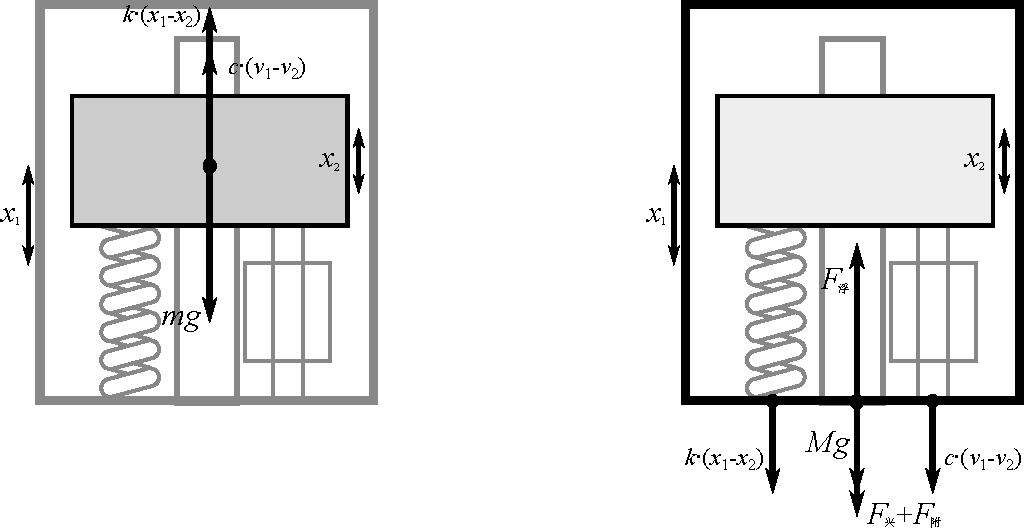
\includegraphics[width=11cm]{fig/force-analysis.pdf}
    \caption{对振子和浮子进行受力分析。为制图方便,未画出完整的浮子壳体}
    \label{force-analysis}
\end{figure}

我们需要确定起始时装置的深度。
记装置静止时受到的总浮力为 $F_\text{浮总}$,水的密度为 $\rho$,装置在水中漂浮时排水体积为 $V_\text{排总}$,则有
\begin{equation}
    \left\{
    \begin{aligned}
        & F_\text{浮总}=\rho gV_\text{排总} \\
        & (m+M)g=F_\text{浮总}
    \end{aligned}
    \right.
\end{equation}
代入附件 4 的数据容易求得 $V_\text{排总}\approx7.121\,\mathrm{m}^3$。
另一方面,考虑浮子下方锥体的体积,有 $V_\text{锥}=\dfrac{1}3\uppi r^2h\approx0.837\,\mathrm{m}^3$。显然,水没过了整个锥体部分,水面在浮子的柱体部分。此时,浮子因在液面中上升下降所造成的浮力变化 $\Delta F_\text{浮}=\rho g\Delta V_{排}=\rho gA\Delta x_1$,其中 $\Delta x_1$ 为浮子没入液面深度的变化量,$A$ 是圆柱的横截面面积。
从而有
\begin{equation}
    F_\text{浮}=F_\text{浮总}+\Delta F_\text{浮}=F_\text{浮总}-\rho gAx_1
    \label{floating}
\end{equation}

联立 \eqref{oscilator}—\eqref{floating} 式,我们可以消去 $mg$、$Mg$、$F_\text{浮}$ 和 $x_0$ 几项,得到
\begin{equation}
    \left\{
    \begin{aligned}
        &  m\dfrac{\dif^2x_2}{\dif t^2}=k(x_1-x_2)+c(\dfrac{\dif{x_1}}{\dif{t}}-\dfrac{\dif{x_2}}{\dif{t}}) \\
        &  M\dfrac{\dif^2x_1}{\dif t^2}=F-k(x_1-x_2)-c(\dfrac{\dif{x_1}}{\dif{t}}-\dfrac{\dif{x_2}}{\dif{t}})-\rho gAx_1-c_0\dfrac{\dif{x_1}}{\dif{t}}-m_0\dfrac{\dif^2 x_1}{\dif t^2}
    \end{aligned}
    \right.
    \label{chui-dang}
\end{equation}
式 \eqref{chui-dang} 就是关于浮子和振子垂荡运动的微分方程组。
考虑装置启动前静止,$t=0$ 时,有初值
\begin{equation}
    \left\{
    \begin{aligned}
        & x_1=x_2=0 \\
        & \dfrac{\dif x_1}{\dif t}=\dfrac{\dif x_2}{\dif t}=0
    \end{aligned}
    \right.
\end{equation}
求解这个初值问题,我们就能解出此题。

\subsubsection{问题求解}

根据附件 3 和附件 4,我们查得式 \eqref{chui-dang} 中的各个常数值如表 \ref{consts-1} 所示。
\begin{table}[htbp]
    \centering
    \begin{tabular}{cc}
        \toprule
        符号 & 常数的值 \\
        \midrule
        $M$ & \N{4866}\,kg \\
        $m$ & \N{2433}\,kg \\
        $k$ & \N{250000}\,$\mathrm{N}\cdot\mathrm{m}$ \\
        $\rho$ & \N{1025}\,$\mathrm{kg}/\mathrm{m}^3$ \\
        $g$ & \N{9.8}\,$\mathrm{m}/\mathrm{s}^2$ \\
        $A$ & $\uppi\,\mathrm{m}^2$ \\
        $c_0$ & \N{656.3616}\,$\mathrm{N}\cdot\mathrm{s}/\mathrm{m}$ \\
        $m_0$ & \N{1335.535}\,kg \\
        \bottomrule
    \end{tabular}
    \caption{问题一适用的部分常量}
    \label{consts-1}
\end{table}

同时,对于波浪激励力 $F$ 我们有
\begin{equation}
    F=f\cos(\omega t)
\end{equation}
其中 $f=\N{6250}\,\mathrm{N}$,$\omega=\N{1.4005}\,\mathrm{s}^{-1}$。
而对于阻尼系数 $c$,有
\begin{equation}
    c=\left\{
        \begin{aligned}
            & \N{10000}\,\mathrm{N}\cdot\mathrm{s}/\mathrm{m}, \text{对于情况 1} \\
            & \N{10000}\sqrt{\left|\dfrac{\dif x_1}{\dif t}-\dfrac{\dif x_2}{\dif t}\right|}\,\mathrm{N}\cdot(\mathrm{s}/\mathrm{m})^{3/2}, \text{对于情况 2}
        \end{aligned}
    \right.
\end{equation}

我们使用计算机对这个二元二阶线性初值问题进行数值求解。
对于题设的两种情况,我们均设定求解起点和终点为 0\,s 和 180\,s,以 0.2\,s 为间隔进行求解,得到在这 180\,s(即前 40 个周期)中,振子和浮子各自的位移和速度,如图所示。

完整的求解结果,我们已经存放在 \verb|result1-1.xlsx| 和 \verb|result1-2.xlsx| 文件中。其中,10\,s,20\,s,40\,s,60\,s,100\,s 时的数据如表所示。

\subsection{问题二}

\subsubsection{输出功率的推导}

波浪能系统的输出功率来自于 PTO 的阻尼力做功。
在 $t$ 时刻,设 PTO 的阻尼力为 $F_\text{PTO}$,记瞬时输出功率为 $P(t)$,则
    \begin{align}
        & F_\text{PTO}=c|v_1-v_2| \\
        & P(t)=F_\text{PTO}\Delta v=c(v_1-v_2)^2
    \end{align}
其中 $v_1$、$v_2$ 是浮子和振子的速度。
得到瞬时功率之后,将其在一段时间内累加(积分)并取平均值,即可得到平均输出功率
\begin{equation}
    \bar{P}=\dfrac{1}{T}\int\limits_0^TP(t)\dif t\approx\dfrac{1}{T}\sum_{i=1}^n\dfrac{P(t_i)+P(t_{i+1})}{2}\Delta t
\end{equation}
结合问题一计算得到的离散速度、位移与时间的关系,我们容易算出给定条件下的 PTO 输出功率。

\subsubsection{最优参数的选择}

本题需要找出在 (1) $c$ 为常数且 $c\in[0, \num{100000}]\,(\mathrm{N}\cdot\mathrm{s}/\mathrm{m})$ 和 (2) $c=c_r|v_1-v_2|^p$,其中 $c_r\in[0, \num{100000}]\,(\mathrm{N}\cdot(\mathrm{s}/\mathrm{m})^{1/p})$ 和 $p\in[0, 1]$ 为常数的两种情况下,平均输出功率 $\bar{P}$ 的最大值和相应的常数系数。